%%%%%%%%%%%%%%%%%%%%%%%%%%%%%%%%%%%%%%%%%%%%%%%%%%%%%%%%%%%%%%%%%%%%%%%%%%%%%%%
% intro.tex: Introduction to the thesis
%%%%%%%%%%%%%%%%%%%%%%%%%%%%%%%%%%%%%%%%%%%%%%%%%%%%%%%%%%%%%%%%%%%%%%%%%%%%%%%%
\chapter{Introduction}
\label{ch:intro}
%%%%%%%%%%%%%%%%%%%%%%%%%%%%%%%%%%%%%%%%%%%%%%%%%%%%%%%%%%%%%%%%%%%%%%%%%%%%%%%%
The Standard Model of particle physics provides a broad and precise description of physical phenomena at the most fundamental and minute level.  While the performance of the theory is, quite frankly, stunning, the Standard Model does not explain everything.  Dark Matter and neutrino masses being relevant examples.

This thesis details an analysis performed with the CMS collaboration at CERN searching for a ``left-right symmetric'' addition to the Standard Model evidenced by a new right-handed neutrino and right-handed intermediating W boson.

The direct pathway for production of the theorized particles contains too much background to be probed effectively at \CMS.  Instead a two step decay process, producing two leptons and two quarks, is looked for.  The Feynman diagram for this is shown below.
\begin{figure}[!htbp]
    \centering
    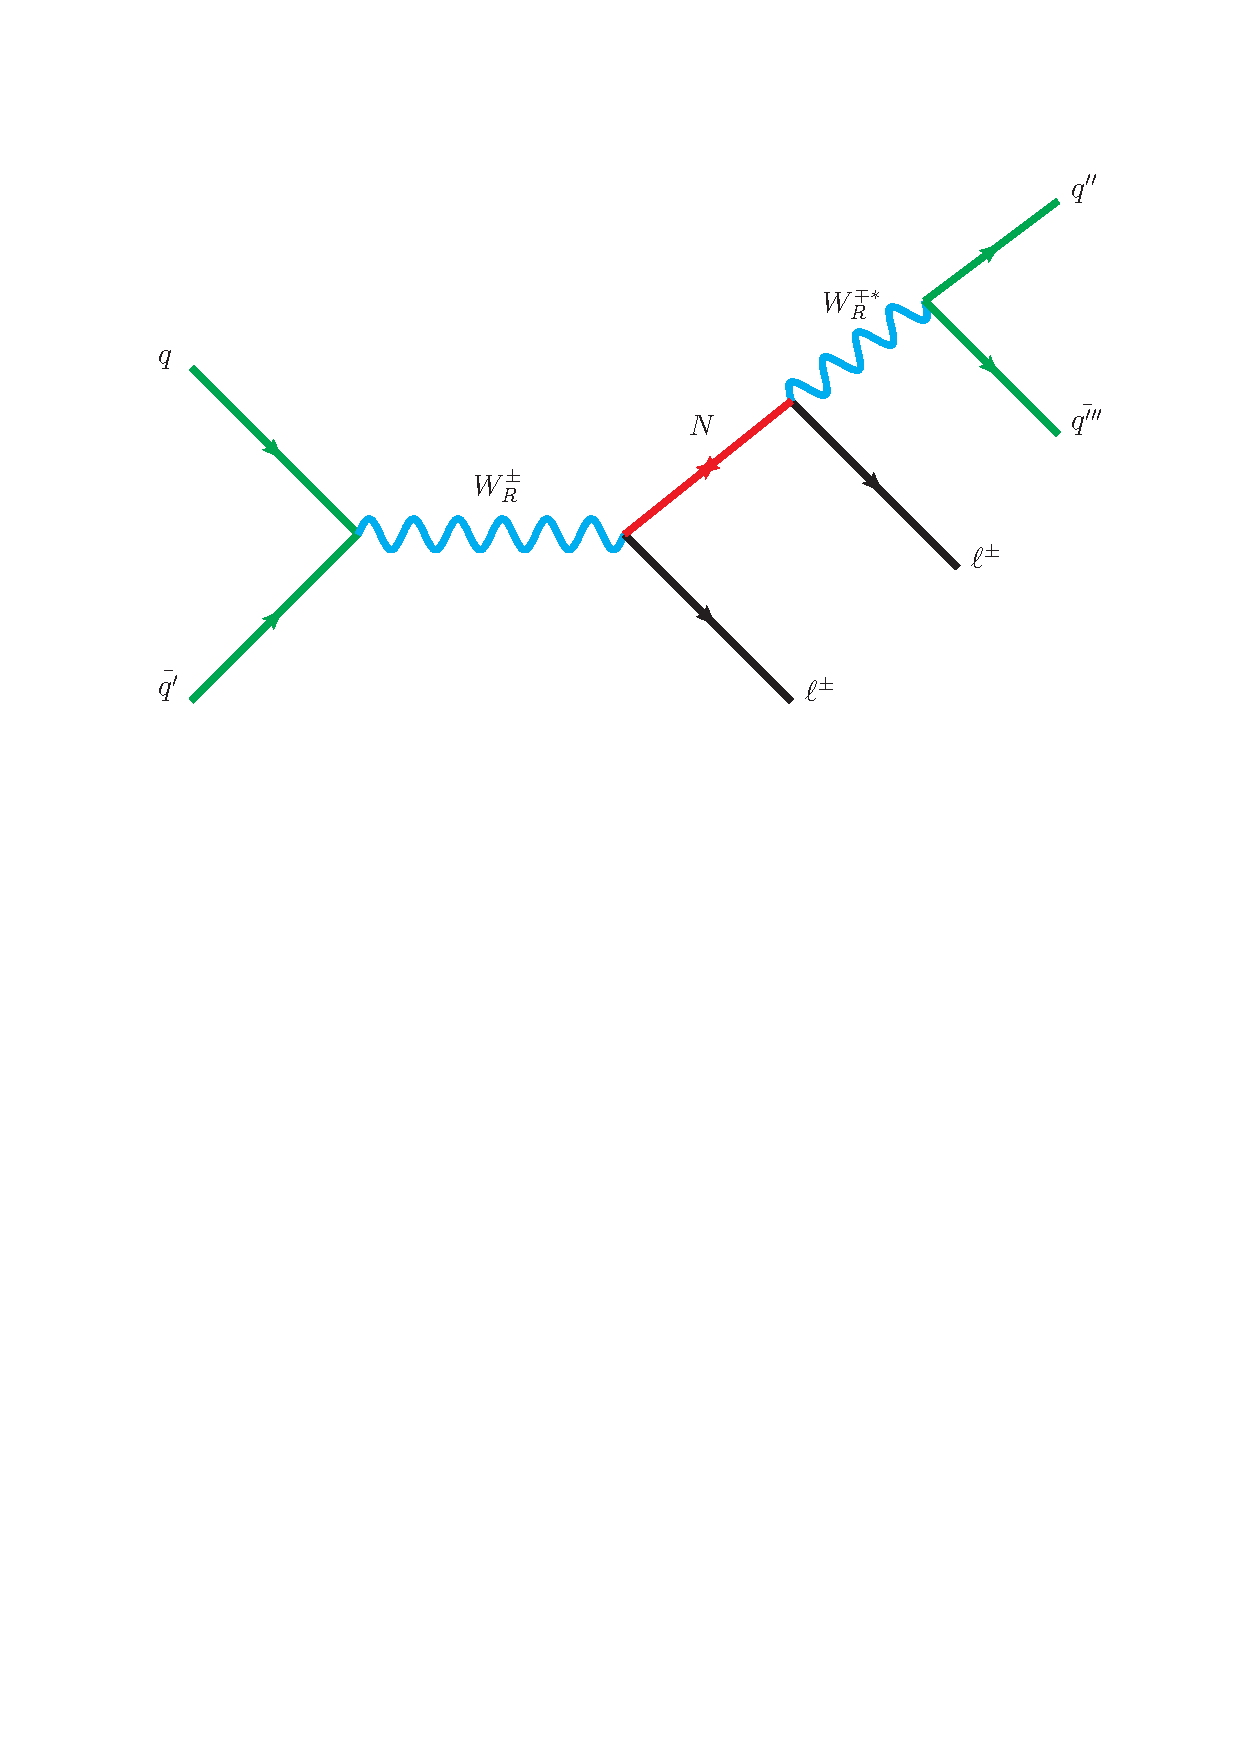
\includegraphics[width=\textwidth]{figures/feynman.pdf}
    \caption[
        The decay process searched for.
    ]{
      The principle Feynman diagram for this analysis.  Two quarks annihilate into a right-handed W boson.  This decays to a lepton and a right-handed neutrino.  This neutrino decays by a virtual right-handed W and another lepton.  This virtual boson decays to quarks, which produce jets.
    }
    \label{fig:mainDiag}
\end{figure}
This analysis combines the past search's technique of identifying all four decay objects with a search relying on the resolution of just three. In addition both 2016 and 2017 data sets, more than doubling the integrated luminosity of past searches.

Analyses have all ready been performed at \rootsseven, \rootseight, and \rootsthirteen \cite{chatrchyan2012a}\cite{osti_1156534}\cite{EXO-17-011} at CMS searching for the lepton, lepton, jet, and jet signature.  While these analyses have excluded certain ranges of neutrino and W boson mass, there remains a possibility that the four particle decay signature is not completely visible because the neutrino is, while heavy, much heavier than the W boson.  In this case, the first muon and right-handed neutrino in the decay chain decay relatively opposite of each other.  This neutrino, carrying significant momentum, results in the next particles in the decay being Lorentz boosted together in the lab frame.  As a result, these particles can be indistinguishable, or poorly reconstructed.

The event selection in this analysis is divided into two separate regions: boosted and resolved. The boosted event selection reconstructs the event with a high energy muon and large jet containing a muon with a novel isolation.  The mass of the summed Lorentz vectors of these two objects is searched for excesses. In the resolved region, two jets and two muons all physically separated in \deltaR are selected.  These four objects are summed and the mass of the result is searched. Both of these selections are designed to reconstruct a signal well, control for backgrounds, and remain orthogonal to each other, allowing for a statistical recombination of the two selection regions. 

This thesis begins with an introduction to the Standard Model and its history in Chapter~\ref{ch:theory}. An introduction to the \CMS detector and the author's work on the \HCAL phase I upgrade are in Chapter~\ref{ch:experiment_chapter}. Details on new boosted-jet techniques are covered in Chapter~\ref{ch:boost}. The focus then shifts to the strategy of the analysis in Chapter~\ref{ch:strategy} and the reconstruction and identification of particles in the analysis in Chapter~\ref{ch:objs}. The estimation of backgrounds is discussed in Chapter~\ref{ch:bg_estim} and the upper confidence limits on the \WR mass are provided in Chapter~\ref{ch:limit_setting}.






%%%%%%%%%%%%%%%%%%%%%%%%%%%%%%%%%%%%%%%%%%%%%%%%%%%%%%%%%%%%%%%%%%%%%%%%%%%%%%%%
